\section[Studentische Mitbestimmung]{Studentische Mitbestimmung~I\\Die verfasste Studierendenschaft und die studentische Selbstverwaltung}
\label{studmit}
\begin{multicols*}{2}
Studierende haben grundsätzlich die Möglichkeit an zwei Gebieten der Universität demokratisch teilzuhaben: in der studentischen und akademischen Selbstverwaltung.
Die verfasste Studierendenschaft ist eine gesetzlich vorgeschriebene Selbstorganisation der Studierenden und bildet somit die studentische Selbstverwaltung. Jede Person, die an der Uni studiert, ist automatisch Teil dieser Studierendenschaft. Sie hat eine große Anzahl an Aufgaben, die im Hochschulgesetz festgeschrieben sind, sowie finanzielle Mittel von mehr als Zehn Millionen Euro jährlich. 
Einmal im Jahr finden die studentischen Wahlen statt, wo z.B. das Studierendenparlament und die Fachschaftsvertretungen neu gewählt werden. 



\bigskip
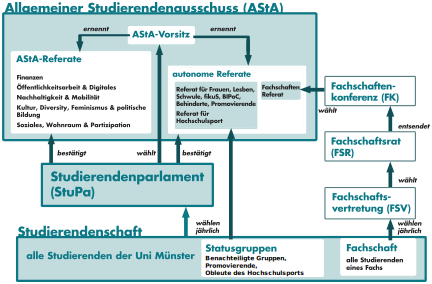
\includegraphics[width=\columnwidth]{res/verfasste_studierendenschaft_neu.pdf}
\bigskip


\subsection{Das Studierendenparlament}
Das StuPa wird einmal im Jahr gewählt und ist -- nun ja -- das Parlament der Studierendenschaft. Das StuPa ist das ranghöchste Gremium in der Studierendenschaft. Zur Wahl des StuPas treten jedes Mal etwa ein dutzend Listen an, bei denen bei manchen auch Parallelen zu den Parteien auf Land und Bundesebene erkennbar sind. In diesen Listen ist es interessierten Leuten möglich, hochschulpolitisch aktiv zu werden. 
Die wichtigste Aufgabe des StuPa ist den AStA zu wählen, welcher die "Regierung" der Studierendenschaft bildet. Die geschieht durch die Bildung von Koalitionen der Listen, welche gemeinsam die absolute Mehrheit an Mandaten im Parlament haben. Das StuPa tagt im 1-2 Wochentakt und ist öffentlich. 


\subsection{Der AStA}
Der Allgemeine Studierenden-Ausschuss ist so etwas wie die Regierung der Studierendenschaft. Er vertretet sie nach außen, verwaltet die finanziellen Mittel und ist in unterschiedliche Referate gegliedert, welche man im Entfernten als Äquivalent zu den Ministerien auf Landes- oder Bundesebene sehen kann.

Von den Geldern der Studierendenschaft werden solidarisch für alle das Semesterticket und die Serviceangebote (siehe Kasten rechts) des AStA finanziert. Die finanziellen Mittel der Fachschaften, von denen zum Beispiel O-Wochen finanziert werden, kommen de Jure ebenfalls aus diesen Geldern. Zum AStA gehören außerdem autonome Referate. Diese werden von der jeweiligen Statusgruppe gewählt und arbeiten daran, das Studium und die Lebensbedingungen für diese Gruppe besser zu gestalten.


\subsection{Die Fachschaftsgremien}
Die Fachschaftsvertretungen~(FSV) werden jährlich zusammen mit dem StuPa gewählt.
Die Aufgabe einer FSV ist die Wahl und Kontrolle des jeweiligen Fachschaftsrats~(FSR), der die Tagesgeschäfte leitet.
Die FSV wird von allen Mitgliedern einer Fachschaft~(FS) gewählt.


Zur FS (Fachschaft) gehören in der Physik alle für einen Studiengang der Physik eingeschriebenen Studierenden, also wahrscheinlich auch der Leser dieses Heftes. Sie ist mit ihren Gremien (FSV, FSR, \dots) Teil der Studierendenschaft. 
Das Wort Fachschaft steht allerdings auch umgangssprachlich für:
\begin{itemize}
	\item den Fachschaftsrat, welcher den Hauptteil der Gremienarbeit, d.h. die Vertretung studentischer Interessen in den Gremien des Fachbereichs, leistet und auch die O-Woche organisiert, das Sommerfest plant und Klausuren/Prüfungsprotokolle verleiht. Er steht über die Fachschaftenkonferenz mit anderen Fachschaften in Kontakt.
Dieser ist meistens gemeint, wenn jemand von "der Fachschaft" spricht.
	\item den Fachschaftsraum am Eingang der KP/TP, wo wir gerne die Studierenden beraten oder Klausuren verleihen.
\end{itemize}
\emph{Die Fachschaft Physik trifft sich aktuell jeden Mittwoch um 18~Uhr im Fachschaftsraum oder online.
Die Sitzungen sind grundsätzlich öffentlich und neue Gesichter sind immer gerne gesehen!}


%\subsection{Das Fachschaftenreferat}
%Das AStA-Fachschaftenreferat ist ein Autonomes Referat des AStA. Es leitet die wöchentliche Fachschaftenkonferenz (FK), in der sich Vertreter der Fachschaftsräte austauschen, und gibt Hilfestellungen für Fachschaften.


\fibelsig{Jan k., Benedikt B.}
\end{multicols*}


\clearpage


\section*{Studentische Mitbestimmung~II\\Die universitären Strukturen und die akademische Selbstverwaltung}
\begin{multicols*}{2}
\begin{quote}
	\textit{Wäre es da nicht doch einfacher, die Regierung löste das Volk auf und wählte ein anderes?}

	\hfill--- Bertold Brecht
\end{quote}
Die Universität selbst ist ebenfalls demokratisch aufgebaut. Dabei werden die Gremien durch die Statusgruppen der Universität, die Studierenden, die Mitarbeiter und die Professoren nach festen Verhältnissen gebildet; die Entsendung geschieht jeweils durch Wahl innerhalb der Statusgruppe.
Die Professoren haben in der Regel absolute Mehrheit. Seit einigen Jahren werden die wichtigsten Entscheidungen im Hochschulrat getroffen, welcher viele externe Mitglieder beinhaltet.


\includegraphics[width=\columnwidth]{res/uni_strukturen.png}


\subsection{Die Fachbereichsräte}
Der FBR ist an einem Fachbereich, also auch in der Physik, das wichtigste Gremium.
Hier wird über die wichtigen Entscheidungen des Dekanats abgestimmt sowie über Berufungen Kommissionen eingerichtet und der Studienbeirat eingesetzt, um die Prüfungsordnungen und deren stetige Verbesserung zu diskutieren.
Die studentischen FBR-Mitglieder (3 reguläre Mitglieder und 3 Stellvertreter) werden im Sommersemester zeitgleich mit den Wahlen der verfassten Studierendenschaft von den Studierenden am Fachbereich gewählt.
Sie stehen euch gerne mit Rat zur Verfügung; ihr könnt sie, wie auch die studentischen Mitglieder des Studienbeirats, über die Fachschaft erreichen, um auf Verbesserungen oder Missstände im Studium hinzuweisen.


\subsection{Der Senat}
Der Senat ist das wichtigste Gremium der akademischen Selbstverwaltung; hier werden Entscheidungen über Berufungen von Professoren, die Prüfungsordnungen der Fachbereiche und vieles weitere, was die gesamte Uni betrifft, getroffen.
So wird hier auch der Haushaltsplan der Universität von der eingesetzten Finanzkommission erstellt.
Die Senatswahl wird ebenfalls meistens gemeinsam mit den anderen Wahlen abgehalten.


\begin{center}
	% Länge „\fboxsep“: Abstand zwischen Inhalt und Rahmen
	\setlength{\fboxsep}{2mm}
	\framebox[\columnwidth]{
	\begin{minipage}{0.95\columnwidth}
		\setlist[itemize]{label={}, nosep, topsep=\smallskipamount, itemsep=\smallskipamount, after={\smallskip}, leftmargin=1.5em}
		\begin{center}
			\large\textbf{Service des AStA}
		\end{center}
		
		\medskip
				
		Der aktuelle AStA bietet folgende Service an:
				
		\smallskip

		\textit{Verleih und Nachhaltigkeit:}
		\begin{itemize}			
			\item Lastenfahrrad-Verleih
			\item Bulli-Verleih
			\item Laptop-Verleih	
			\item Musikanlagen-Verleih		
			\item Grüne Kiste	
			\item Kooperation mit Leihothek Münster		
		\end{itemize}

		\textit{Soziales, Finanzierung und Mobilität:}
		\begin{itemize}
			\item Beglaubigte Kopien von Dokumenten
			\item BAföG- und Sozialberatung
			\item Semesterticket und Kultursemesterticket
			\item Beitragserstattungen und Sozialdarlehen
			\item kostenlose professionelle Rechtsberatung
			\item Babysitting- und Wohnbörse 
			\item Kooperation mit Fahrradwerkstatt Hafenstraße 34
			\item Sprachkurse
		\end{itemize}

		\textit{kostenlose Fahrradpumpen} auf \url{https://www.asta.ms/fahrradreperaturstationen}
		
		\textit{AStA-Druckerei:}
		\begin{itemize}
			\item druckt Abschlussarbeiten, Poster etc.
		\end{itemize}
			
		\textit{Wohnbörse} auf \url{https://www.asta.ms/wohnboerse}
		
		\textit{Babysittingbörse} auf \url{https://www.asta.ms/babysittingboerse}

		\medskip
		\small
		Weitere Informationen auf: \url{https://www.asta.ms}
	\end{minipage}
	}
\end{center}


\subsection{Das Rektorat}
Das Rektorat ist die Leitung der Uni, welche auch die Verwaltung und das Studierendensekretariat betreut.
Aktueller Rektor ist Herr Prof.\ Johannes Wessels (aus dem Institut für Kernphysik).
Das Rektorat wird unter Aufsicht des Senats vom Hochschulrat gewählt und führt die Vorgaben des Senats und Hochschulrates aus.


\subsection{Der Hochschulrat}
Der Hochschulrat~(HSR) gibt die Ziele und Richtungen der Universität vor.
Bisher gibt es keine Möglichkeit, bei der Entscheidungsfindung des HSR einzugreifen, und so muss sich selbst der von den Mitgliedern der Uni gewählte Senat nach den Entscheidungen richten.


\fibelsig{Jan k., Benedikt B.}
\end{multicols*}

